% Name: Law of cosines
% Description: The height from B splits side b, so the right triangle on the far side gives c² = (a sin γ)² + (b − a cos γ)² = a² + b² − 2ab cos γ.
% Tags: law of cosines, trigonometry, triangle, cosine rule

\usetikzlibrary{angles, quotes, decorations.pathreplacing}

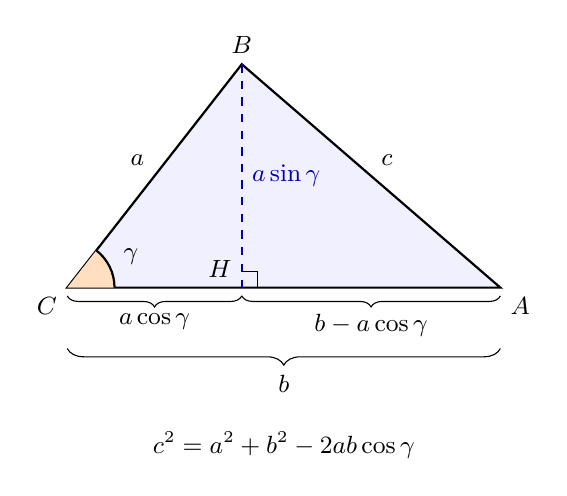
\begin{tikzpicture}[thick, every node/.style={font=\small}]
  % a = 3.6 at gamma = 52 degrees: B = (3.6 cos 52, 3.6 sin 52) = (2.2164, 2.8369); H is the foot of the height on CA
  \coordinate[label=below left:$C$] (C) at (0,0);
  \coordinate[label=below right:$A$] (A) at (5.5,0);
  \coordinate[label=above:$B$] (B) at (52:3.6);
  \coordinate (H) at (B |- C);
  \draw[fill=blue!6] (C) -- (A) -- node[above right] {$c$} (B) -- node[above left] {$a$} cycle;
  \draw[dashed, blue!70!black] (B) -- node[right] {$a \sin\gamma$} (H);
  \pic[draw, thin, angle radius=2mm] {right angle=B--H--A};
  \node[above left] at (H) {$H$};
  \pic[draw, fill=orange!25, angle radius=6mm, "$\gamma$", angle eccentricity=1.5] {angle=A--C--B};
  \draw[decorate, decoration={brace, mirror, amplitude=4pt, raise=3pt}, thin] (C) -- node[below=6pt] {$a\cos\gamma$} (H);
  \draw[decorate, decoration={brace, mirror, amplitude=4pt, raise=3pt}, thin] (H) -- node[below=6pt] {$b - a\cos\gamma$} (A);
  \draw[decorate, decoration={brace, mirror, amplitude=6pt, raise=22pt}, thin] (C) -- node[below=28pt] {$b$} (A);
  \node at (2.75,-2) {$c^2 = a^2 + b^2 - 2ab\cos\gamma$};
\end{tikzpicture}
